Du ziehst einen Schlitten mit einem Kind darauf (zusammen \mO) mit konstanter Geschwindigkeit über ebenen Schnee. Das Seil ist \lSO\ lang, und deine Hand ist \hSO\ höher als die Stelle, an der das Seil am Schlitten befestigt ist. Die Reibungszahl zwischen Schlitten und Schnee beträgt \muGO. Rechne mit \gO.

\begin{center}
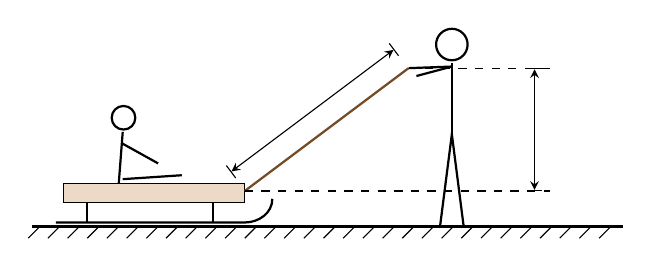
\begin{tikzpicture}[>=stealth]
 \draw[thick] (-0.3,0) -- (7.2,0);
 \foreach \x in {-0.2,0.05,...,7.1} \draw (\x,0) -- ++(-0.15,-0.15);
 \draw[thick] (0,0.05) -- (2.4,0.05) to[out=0, in=-90] (2.75,0.35);
 \draw[thick] (0.4,0.05) -- (0.4,0.3) (2.0,0.05) -- (2.0,0.3);
 \draw[fill=brown!30] (0.1,0.3) rectangle (2.4,0.55);
 \draw[thick] (0.8,0.55) -- (0.85,1.2) (0.85,0.6) -- (1.6,0.65) (0.85,1.05) -- (1.3,0.8);
 \draw[thick, fill=white] (0.86,1.38) circle (0.15);
 \draw[thick, brown!60!black] (2.4,0.45) -- (4.48,2.01);
 \draw[thick] (4.88,0) -- (5.03,1.17) -- (5.18,0);
 \draw[thick] (5.03,1.17) -- (5.03,2.08);
 \draw[thick, fill=white] (5.03,2.31) circle (0.2);
 \draw[thick] (5.03,2.03) -- (4.48,2.01);
 \draw[thick] (5.03,2.03) -- (4.58,1.91);
 \draw[|<->|, thin] (2.22,0.69) -- node[above left] {\lSO} (4.3,2.25);
 \draw[dashed, thin] (2.4,0.45) -- (6.28,0.45) (4.48,2.01) -- (6.28,2.01);
 \draw[|<->|, thin] (6.08,0.45) -- node[right] {\hSO} (6.08,2.01);
\end{tikzpicture}
\end{center}

\begin{abcliste}
\abc
Wie stark musst du ziehen?

\abc
Wie gross ist die Normalkraft auf den Schlitten?
\end{abcliste}
